\documentclass{article}

\usepackage[utf8]{inputenc}
\usepackage[T1]{fontenc}
\usepackage{hyperref}
\usepackage{url}
\usepackage{booktabs}
\usepackage{amsmath}
\usepackage{amsfonts}
\usepackage{graphicx}
\usepackage{caption}
\usepackage{float}
\graphicspath{{./}{./images/}{./TP 1.1/}{./TP 1.1/images/}}

\title{TP 1.1 - Simulación de una Ruleta}

\author{
  Valentino Nicola \\
  49831 \\
  \texttt{valenicola02@gmail.com} \\
  \and
  Augusto Lescano\\
  50422 \\
  \texttt{augustolescano15@gmail.com} \\
  \and
  Lucas Viguera\\
  46875 \\
  \texttt{lucas.viguera2001@gmail.com} \\
  \and
  Facundo Ramírez \\
  48808 \\
  \texttt{facundomrb@gmail.com} \\
}

\date{}

\begin{document}

\maketitle

\begin{abstract}
El presente trabajo analiza, desde una perspectiva probabilística y computacional, el comportamiento de una ruleta ideal europea mediante simulación. El objetivo no es únicamente describir resultados observados, sino verificar analíticamente si los estimadores muestrales obtenidos por simulación convergen a los parámetros teóricos de una distribución uniforme discreta sobre los valores de 0 a 36. Para ello se comparan múltiples corridas independientes, se estudian medidas acumuladas y se contrasta la evidencia empírica con los valores teóricos esperados.
\end{abstract}

\section{Introducción}
La ruleta suele entenderse como un juego puramente azaroso; sin embargo, desde el punto de vista matemático constituye un sistema estocástico con estructura probabilística bien definida. En una ruleta ideal europea, cada número entre 0 y 36 posee igual probabilidad de ocurrencia, por lo que la distribución subyacente es uniforme discreta.

En este marco, la simulación computacional permite contrastar teoría y evidencia empírica. A medida que aumenta el número de observaciones, las métricas muestrales deberían aproximarse a sus valores teóricos. Esta expectativa se encuentra respaldada por la Ley de los Grandes Números, que afirma que, bajo repeticiones independientes de una misma experiencia aleatoria, los promedios y frecuencias relativas tienden a estabilizarse alrededor de sus valores esperados.

A partir de esta idea, el trabajo se orienta a responder una pregunta concreta de investigación: \textbf{¿en qué medida los estimadores muestrales obtenidos mediante simulación de una ruleta ideal convergen a los parámetros teóricos de la distribución uniforme discreta al aumentar el número de tiradas?}

Responder esta pregunta permite pasar de una descripción de resultados a una verificación analítica del modelo. Además, el problema tiene valor aplicado: en contextos de \textit{e-commerce}, métricas como tasa de conversión, ticket promedio o dispersión entre campañas también se estiman a partir de muestras aleatorias y exhiben comportamientos de convergencia análogos. En ese sentido, la ruleta funciona como un caso controlado para comprender cómo evolucionan métricas observables a medida que se acumulan datos.

\section{Conceptos teóricos empleados}

\subsection{Población}
Se denomina población al conjunto total de elementos sobre los que se desea inferir. En este caso, la población está compuesta por todas las posibles tiradas de una ruleta ideal, lo cual puede modelarse como una sucesión potencialmente infinita de ensayos independientes.

\subsection{Muestra}
Una muestra es un subconjunto finito de observaciones extraídas de la población. En este trabajo, cada corrida constituye una muestra de tiradas de ruleta de tamaño finito.

\subsection{Modelo probabilístico}
Sea la variable aleatoria discreta $X$ definida como el resultado de una tirada de ruleta europea ideal. Entonces:

\begin{equation}
X \sim U\{0,1,2,\dots,36\}
\end{equation}

y, en consecuencia,

\begin{equation}
P(X = k) = \frac{1}{37}, \qquad k \in \{0,1,2,\dots,36\}
\end{equation}

Dado que todos los resultados son equiprobables, el valor esperado de la variable es:

\begin{equation}
E(X) = \frac{0 + 36}{2} = 18
\end{equation}

La varianza teórica de una distribución uniforme discreta con 37 valores consecutivos es:

\begin{equation}
\mathrm{Var}(X) = \frac{37^2 - 1}{12} = 114
\end{equation}

Por lo tanto, el desvío estándar teórico resulta:

\begin{equation}
\sigma = \sqrt{114} \approx 10.6771
\end{equation}

Este modelo teórico constituye el punto de referencia para todo el análisis empírico desarrollado posteriormente.

\subsection{Frecuencia relativa}
La frecuencia relativa del número elegido mide la proporción de veces que ocurre dicho evento respecto del total de observaciones acumuladas:

\begin{equation}
f_i = \frac{n_i}{N}
\end{equation}

donde $n_i$ representa la cantidad de ocurrencias del evento y $N$ el número de tiradas observadas hasta ese instante.

\subsection{Promedio muestral}
El promedio muestral acumulado para una corrida de tamaño $n$ se define como:

\begin{equation}
\bar{x}_n = \frac{1}{n} \sum_{i=1}^{n} x_i
\end{equation}

\subsection{Varianza y desvío estándar muestrales}
Para mantener consistencia matemática, en el análisis empírico se utiliza la varianza muestral:

\begin{equation}
s_n^2 = \frac{1}{n - 1} \sum_{i=1}^{n} (x_i - \bar{x}_n)^2
\end{equation}

El desvío estándar muestral correspondiente es:

\begin{equation}
s_n = \sqrt{s_n^2}
\end{equation}

Esta elección es coherente con la implementación computacional utilizada en el script, donde media, varianza y desvío se calculan de manera incremental mediante el algoritmo de Welford.

\subsection{Ley de los Grandes Números}
La Ley de los Grandes Números establece que, al repetir una experiencia aleatoria independiente un número suficientemente grande de veces, los promedios y las frecuencias relativas convergen hacia sus valores esperados. Aplicada a este trabajo, dicha ley sugiere que:

\begin{itemize}
    \item la frecuencia relativa del número 17 debería aproximarse a $1/37$;
    \item el promedio acumulado de las tiradas debería aproximarse a $18$;
    \item la varianza y el desvío estándar muestrales deberían estabilizarse alrededor de $114$ y $\sqrt{114}$, respectivamente.
\end{itemize}

La simulación permite verificar empíricamente si esta convergencia efectivamente ocurre y con qué velocidad se manifiesta bajo distintos tamaños muestrales.

\section{Metodología}

\subsection{Objetivo de verificación}
El diseño experimental se construyó para responder la pregunta de investigación planteada en la introducción: verificar si los estimadores muestrales producidos por la simulación convergen a los parámetros teóricos del modelo probabilístico de una ruleta ideal.

\subsection{Implementación computacional}
El programa fue desarrollado en Python. La generación de tiradas se realizó con la librería estándar \texttt{random}, basada en el generador pseudoaleatorio Mersenne Twister. Para facilitar la reproducibilidad de resultados comparables, se fijó una semilla constante (\texttt{seed = 42}).

Con el fin de mejorar la eficiencia computacional y evitar recalcular o almacenar la muestra completa en cada paso, la media y la varianza muestral se obtuvieron mediante el algoritmo incremental de Welford. Esta decisión permite trabajar con volúmenes elevados de datos manteniendo estabilidad numérica.

\subsection{Diseño experimental}
Se definió un patrón común para ambos experimentos:

\begin{enumerate}
    \item se fijó un número de interés ($17$) para estudiar su frecuencia relativa acumulada;
    \item se ejecutaron múltiples corridas independientes;
    \item en cada corrida se registraron, tirada a tirada, la frecuencia relativa acumulada, el promedio acumulado, la varianza muestral acumulada y el desvío estándar muestral acumulado;
    \item finalmente, se compararon los resultados empíricos con sus correspondientes valores teóricos.
\end{enumerate}

Bajo este mismo patrón, se trabajó con dos escalas distintas:

\begin{itemize}
    \item \textbf{Experimento 1:} 1.000 corridas independientes de 30.000 tiradas cada una.
    \item \textbf{Experimento 2:} 300 corridas independientes de 100.000 tiradas cada una.
\end{itemize}

Esta estructura permite estudiar simultáneamente dos cuestiones: la convergencia intra-corrida de cada estimador y la dispersión inter-corridas al aumentar el tamaño muestral.

\subsection{Métricas por corrida}
Para cada corrida $j$ se construyeron cuatro series acumuladas:

\begin{itemize}
    \item frecuencia relativa del número 17, $f_n^{(j)}$;
    \item promedio acumulado, $\bar{x}_n^{(j)}$;
    \item varianza muestral acumulada, $s_{n}^{2\,(j)}$;
    \item desvío estándar muestral acumulado, $s_n^{(j)}$.
\end{itemize}

Luego, para cada valor de $n$ se calculó el promedio entre corridas de cada métrica, junto con una banda de dispersión delimitada por los percentiles 10 y 90. De esta manera, el análisis no se limita a una única trayectoria, sino que resume tendencia central y variabilidad entre corridas.

\subsection{Visualización e interpretación gráfica}
Los gráficos generados por el script adoptan un formato analítico coherente con la pregunta de investigación:

\begin{itemize}
    \item cada métrica se representa en un \textbf{subplot} específico;
    \item las corridas individuales se muestran mediante líneas finas y transparentes, para evitar saturación visual;
    \item una línea gruesa representa el promedio entre corridas para cada cantidad de tiradas;
    \item una banda sombreada representa el intervalo de dispersión entre los percentiles 10 y 90;
    \item una línea horizontal punteada marca el valor teórico correspondiente.
\end{itemize}

Este tipo de representación permite evaluar simultáneamente convergencia, dispersión y distancia al valor teórico. Por ello, no se trata sólo de “mostrar resultados”, sino de aportar evidencia visual sostenida para verificar la hipótesis de convergencia.

\section{Resultados y discusión}

\subsection{Experimento 1: 1.000 corridas de 30.000 tiradas}
Los valores finales promediados entre las 1.000 corridas, luego de completar las 30.000 tiradas en cada una, se presentan en la Tabla~\ref{tab:exp1}.

\begin{table}[H]
\centering
\small\begin{tabular}{@{}lcccc@{}}
\toprule
\textbf{Métrica} & \textbf{Valor empírico} & \textbf{Valor teórico} & \textbf{Error abs.} & \textbf{Error rel.} \\
\midrule
Frecuencia relativa (17) & 0.0271 & 0.0270 ($1/37$) & 0.0001 & 0.37\% \\
Promedio & 17.9994 & 18.0000 & 0.0006 & 0.0033\% \\
Varianza muestral & 114.0122 & 114.0000 & 0.0122 & 0.0107\% \\
Desvío estándar muestral & 10.6776 & 10.6771 ($\sqrt{114}$) & 0.0005 & 0.0047\% \\
\bottomrule
\end{tabular}
\caption{Resumen cuantitativo del Experimento 1.}
\label{tab:exp1}
\end{table}

Los resultados muestran errores absolutos muy reducidos y errores relativos inferiores al 0.4\% en todas las métricas, con valores particularmente pequeños en promedio, varianza y desvío estándar. En términos analíticos, esto constituye evidencia fuerte de que la simulación reproduce con precisión el comportamiento esperado del modelo uniforme discreto.

La frecuencia relativa del número 17 se ubica en 0.0271, apenas 0.0001 por encima de su valor teórico. El promedio empírico final difiere de 18 en sólo 0.0006 unidades. Más aún, la varianza y el desvío estándar muestrales exhiben errores relativos de 0.0107\% y 0.0047\%, respectivamente. Estas magnitudes son lo suficientemente pequeñas como para atribuir las discrepancias observadas al azar muestral residual y no a sesgos del modelo o del generador pseudoaleatorio.

\begin{figure}[H]
    \centering
    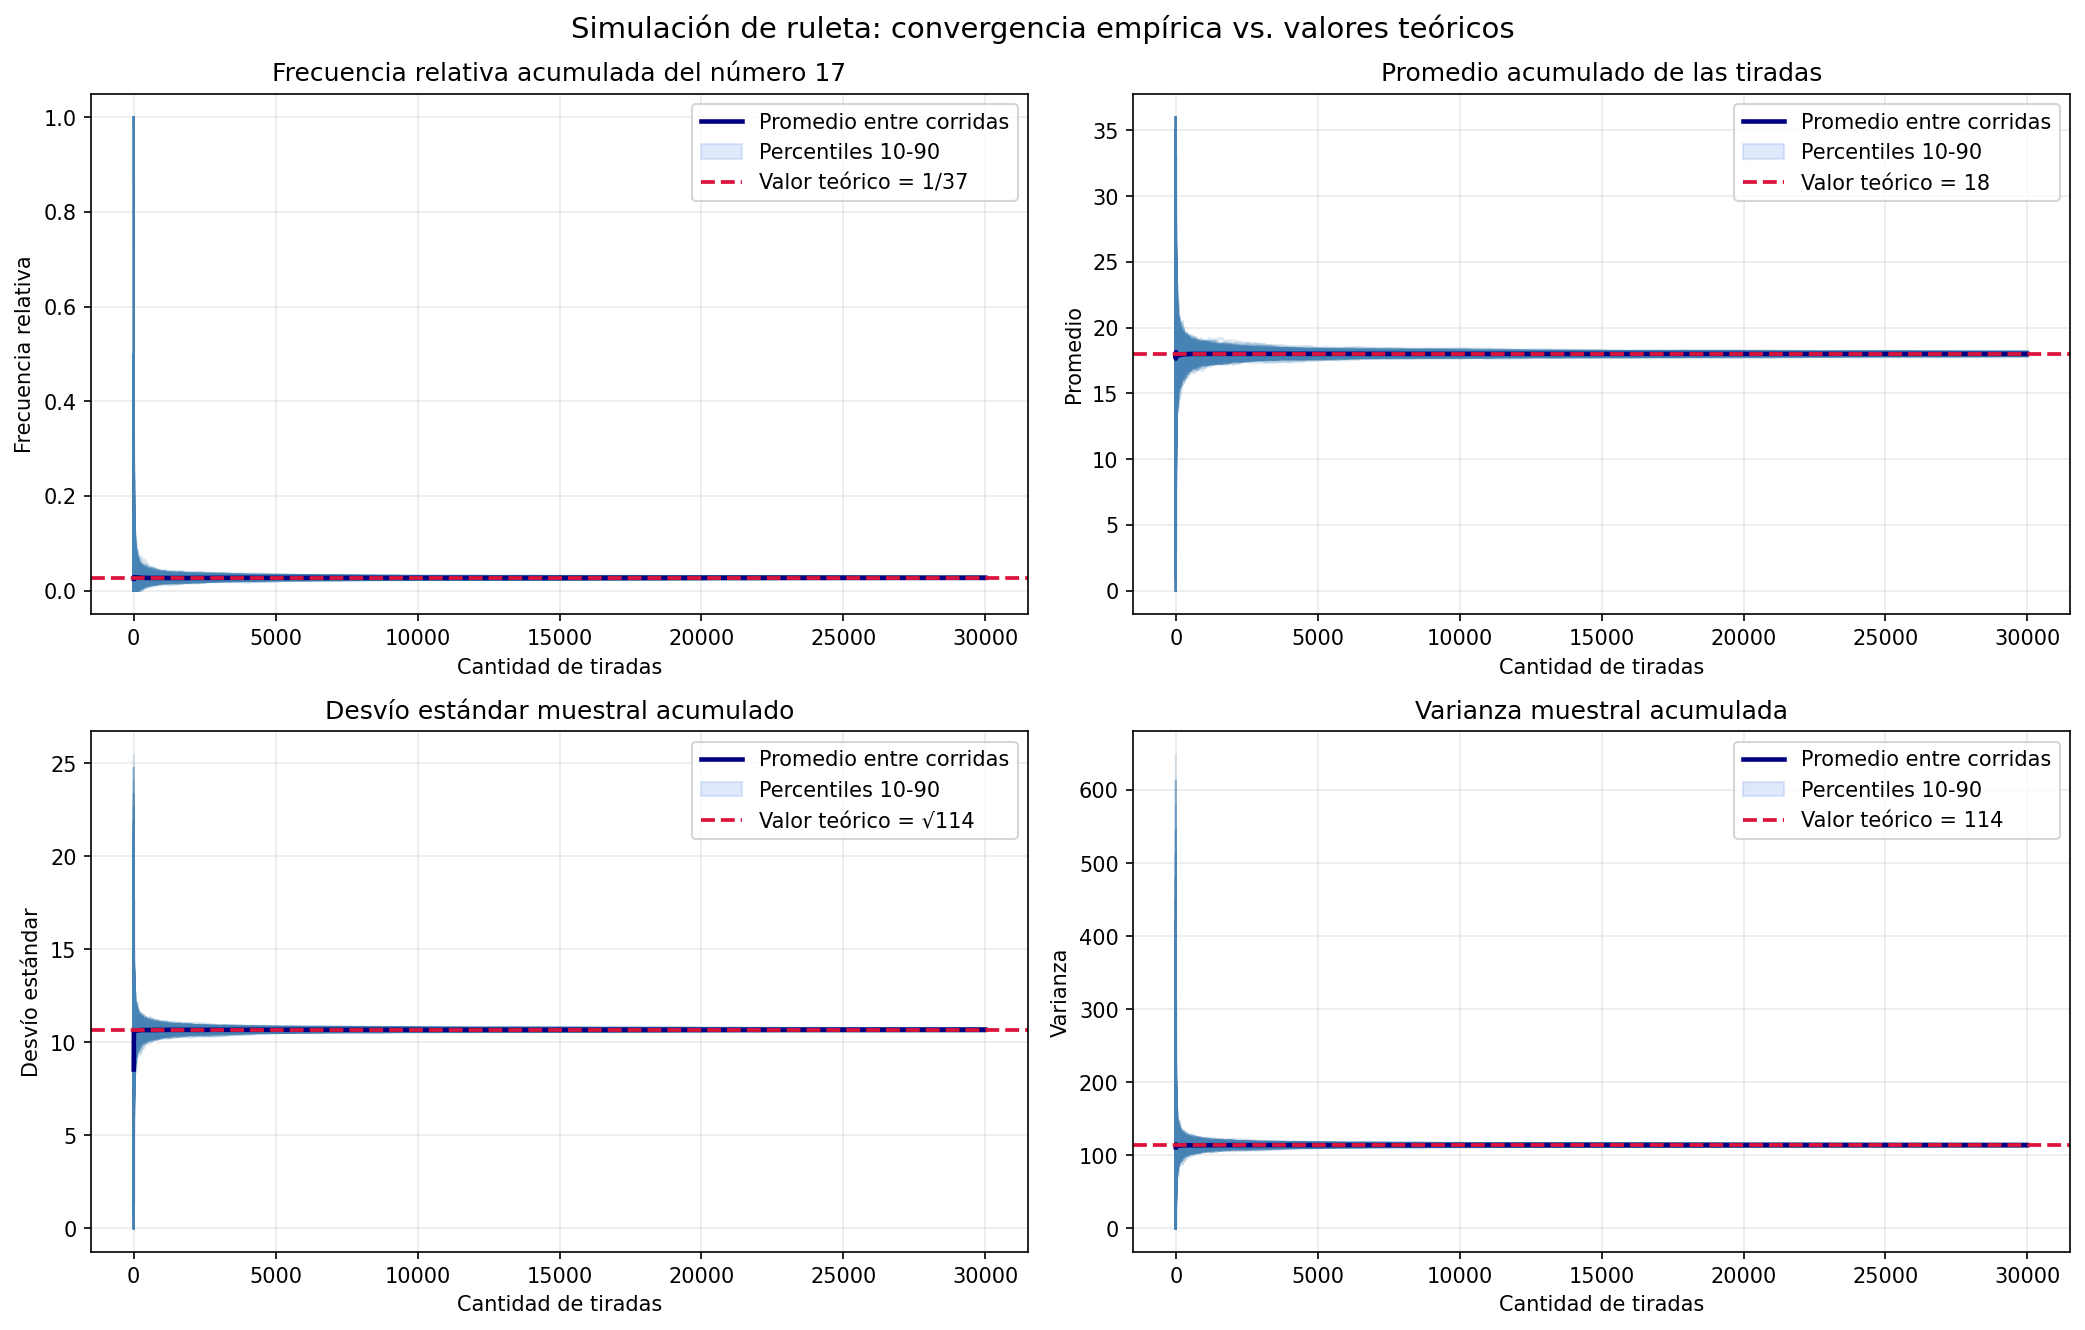
\includegraphics[width=\textwidth]{informe_ruleta1.png}
    \caption{Experimento 1. Cada subplot corresponde a una métrica distinta: frecuencia relativa, promedio, desvío estándar muestral y varianza muestral. Las líneas finas transparentes representan corridas individuales; la línea gruesa representa el promedio entre corridas; la banda sombreada muestra el intervalo entre percentiles 10 y 90; la línea horizontal punteada indica el valor teórico.}
\end{figure}

La interpretación de los gráficos refuerza el análisis numérico. En el subplot de frecuencia relativa, las trayectorias individuales presentan oscilaciones visibles al inicio, pero el promedio entre corridas converge rápidamente hacia $1/37$. En el subplot del promedio, la media acumulada se alinea de manera progresiva con el valor teórico 18. En los subplots de varianza y desvío estándar, la dispersión es inicialmente mayor, pero disminuye con claridad a medida que aumenta el número de tiradas.

La contracción de la banda sombreada es especialmente importante: indica que no sólo el promedio entre corridas converge, sino que también disminuye la heterogeneidad entre corridas independientes. En otras palabras, el aumento del tamaño muestral mejora simultáneamente precisión y estabilidad.

\subsection{Experimento 2: 300 corridas de 100.000 tiradas}
El segundo experimento extiende el horizonte de observación, priorizando un mayor número de tiradas por corrida para estudiar la consolidación de la convergencia a largo plazo. Los valores finales se resumen en la Tabla~\ref{tab:exp2}.

\begin{table}[H]
\centering
\small\begin{tabular}{@{}lcccc@{}}
\toprule
\textbf{Métrica} & \textbf{Valor empírico} & \textbf{Valor teórico} & \textbf{Error abs.} & \textbf{Error rel.} \\
\midrule
Frecuencia relativa (17) & 0.0271 & 0.0270 ($1/37$) & 0.0001 & 0.37\% \\
Promedio & 17.9994 & 18.0000 & 0.0006 & 0.0033\% \\
Varianza muestral & 114.0124 & 114.0000 & 0.0124 & 0.0109\% \\
Desvío estándar muestral & 10.6776 & 10.6771 ($\sqrt{114}$) & 0.0005 & 0.0047\% \\
\bottomrule
\end{tabular}
\caption{Resumen cuantitativo del Experimento 2.}
\label{tab:exp2}
\end{table}

La evidencia cuantitativa sigue siendo plenamente consistente con el modelo teórico. El promedio y el desvío estándar permanecen prácticamente coincidentes con los parámetros esperados, mientras que la varianza conserva un error relativo cercano al 0.01\%. Estos resultados permiten afirmar, de manera precisa y cuantificable, que incluso con menor cantidad de corridas, el aumento del tamaño de cada muestra individual refuerza la estabilidad de los estimadores acumulados.

\begin{figure}[H]
    \centering
    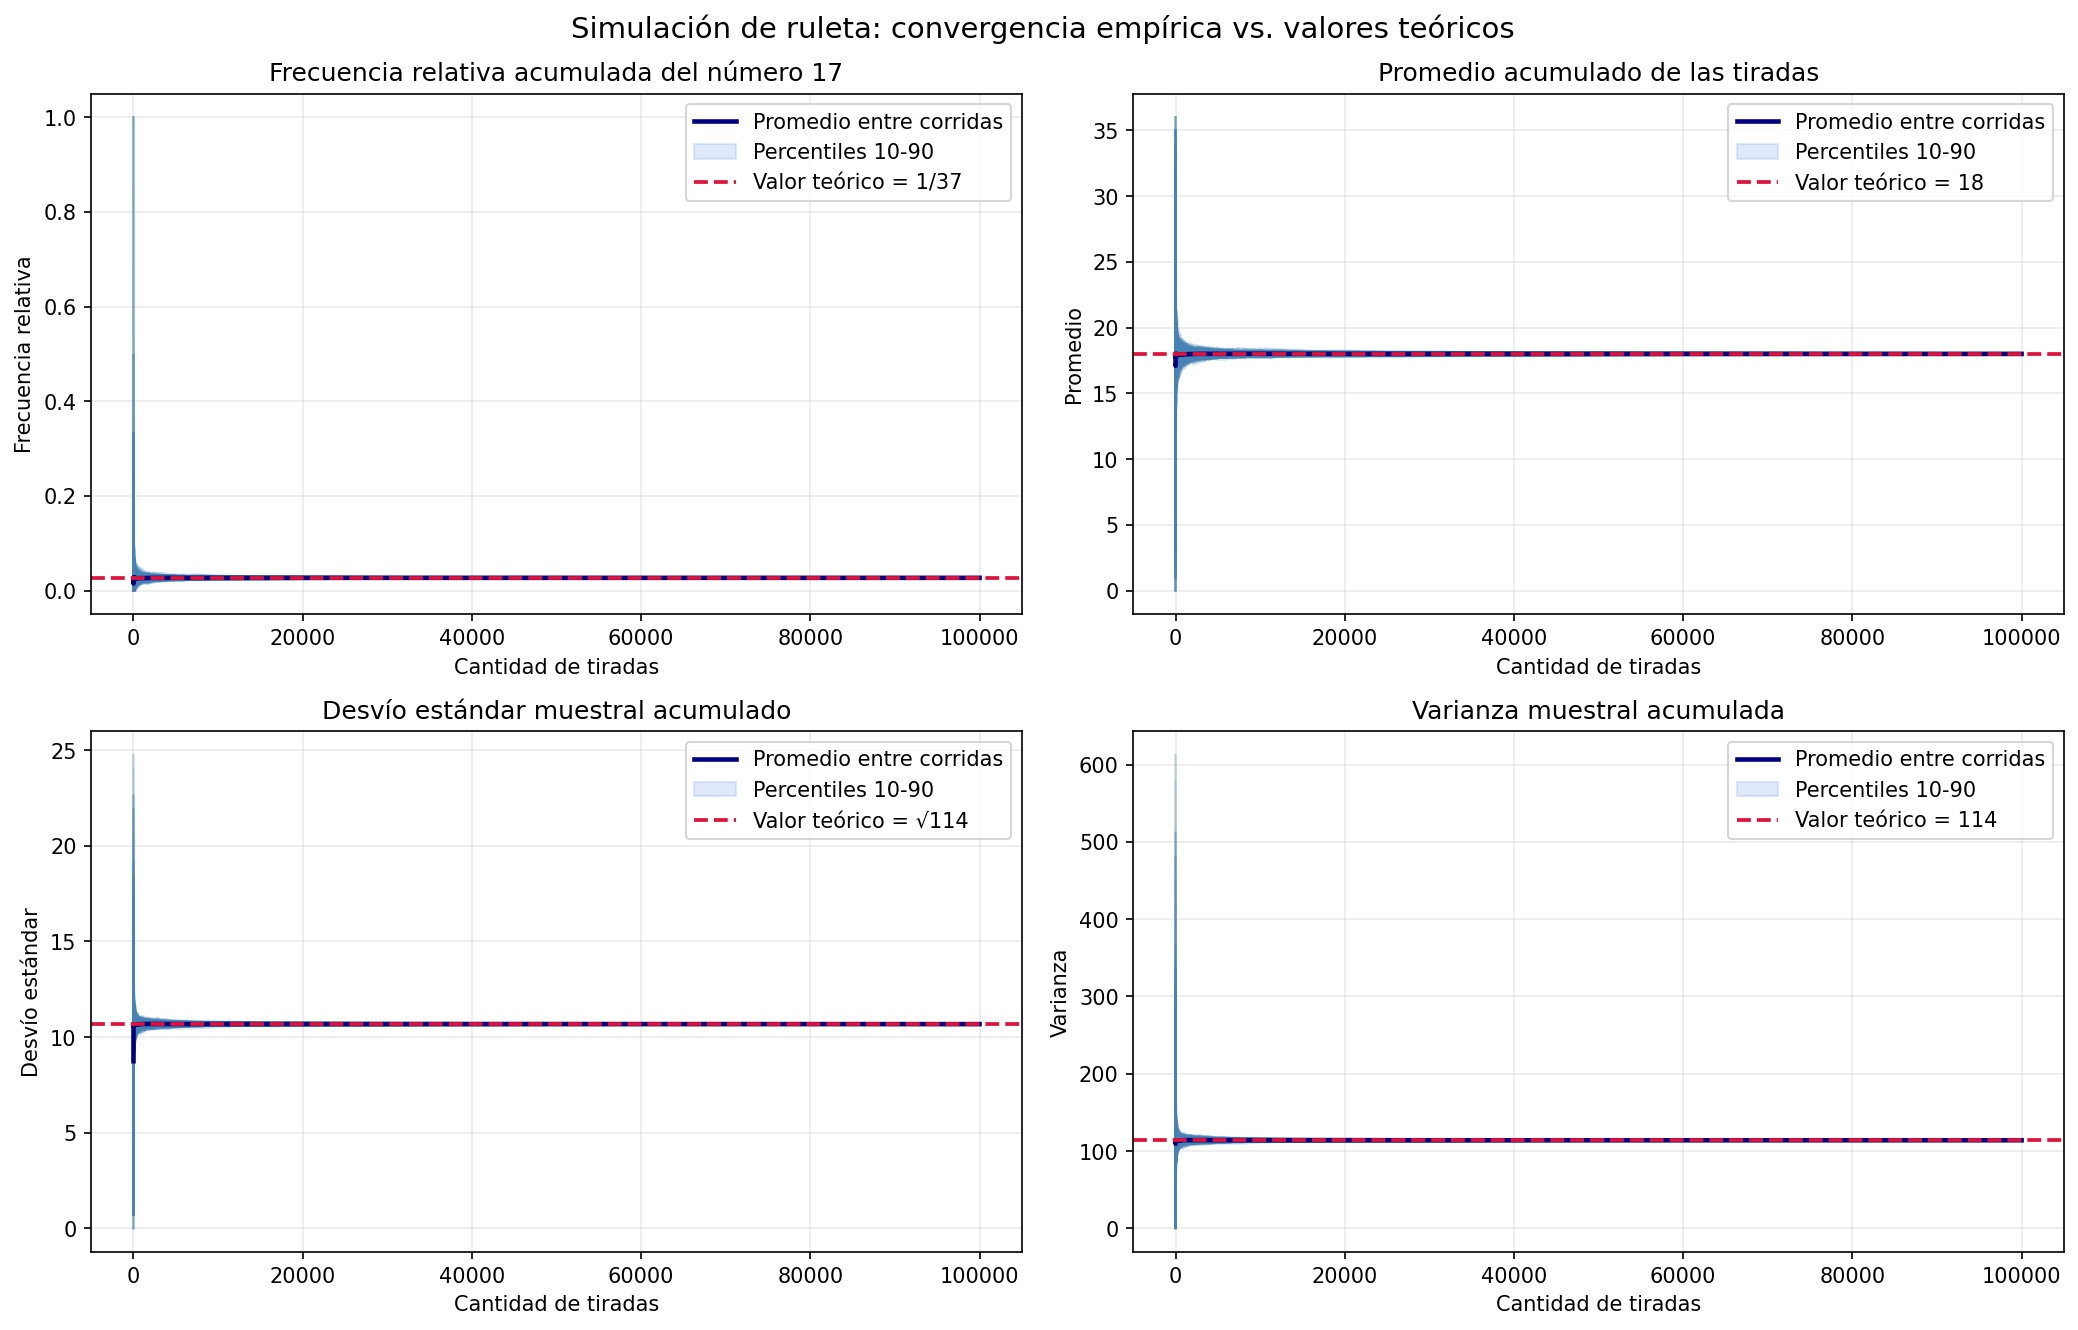
\includegraphics[width=\textwidth]{informe_ruleta2.png}
    \caption{Experimento 2. Se repite la estructura analítica del Experimento 1: un subplot por métrica, corridas individuales transparentes, promedio entre corridas, banda percentil 10--90 y línea horizontal teórica de referencia.}
\end{figure}

Desde el punto de vista gráfico, el segundo experimento muestra una estabilización todavía más marcada. Hacia el tramo final de las 100.000 tiradas, las oscilaciones de las corridas individuales pierden amplitud, la banda de dispersión se comprime y el promedio entre corridas se superpone casi por completo con el valor teórico en los cuatro subplots. Esto constituye una verificación empírica aún más clara de la Ley de los Grandes Números.

\subsection{Comparación entre experimentos}
La comparación entre ambos experimentos permite distinguir dos efectos complementarios. Por un lado, el Experimento 1 ofrece una base más amplia de corridas y, por lo tanto, una excelente caracterización de la variabilidad entre trayectorias. Por otro lado, el Experimento 2, aun con menos corridas, presenta mayor longitud temporal y una estabilización visual más contundente al final del proceso.

En ambos casos, los errores absolutos y relativos son muy bajos, por lo que la respuesta a la pregunta de investigación es afirmativa: \textbf{los estimadores muestrales obtenidos mediante simulación convergen de manera consistente a los parámetros teóricos del modelo probabilístico de la ruleta ideal}. La evidencia que sostiene esta respuesta es doble: numérica, a partir de errores pequeños y cuantificables; y gráfica, a partir del alineamiento entre promedios empíricos, bandas de dispersión decrecientes y líneas teóricas de referencia.

\section{Limitaciones metodológicas}
Aunque la evidencia obtenida es sólida, las conclusiones deben interpretarse dentro del marco del diseño experimental adoptado. En primer lugar, la frecuencia relativa se siguió para un único número específico (17). Dado que el modelo es simétrico, esta decisión es razonable; sin embargo, no equivale a una verificación empírica individual de todos los resultados posibles.

En segundo lugar, el estudio compara únicamente dos configuraciones de tamaño muestral. Esto permite identificar una tendencia clara de convergencia, pero no describe de forma exhaustiva qué ocurre para otros tamaños intermedios o extremos.

En tercer lugar, el modelo supone una ruleta ideal perfectamente uniforme. En consecuencia, el análisis no contempla sesgos físicos, defectos mecánicos ni perturbaciones propias de una ruleta real. Por lo tanto, la validez de las conclusiones es interna al modelo simulado y no debe extrapolarse sin reservas a sistemas físicos concretos.

Expresar estas limitaciones no debilita el trabajo; por el contrario, delimita con precisión el alcance de la evidencia y fortalece la interpretación científica de los resultados.

\section{Conclusión}
La pregunta de investigación planteada fue la siguiente: \textit{¿en qué medida los estimadores muestrales obtenidos mediante simulación de una ruleta ideal convergen a los parámetros teóricos de la distribución uniforme discreta al aumentar el número de tiradas?}

A la luz de los resultados, la respuesta es afirmativa. Tanto en el experimento de 30.000 tiradas como en el de 100.000 tiradas, la frecuencia relativa, el promedio, la varianza muestral y el desvío estándar muestral convergen hacia los valores teóricos esperados. Esta afirmación no se sostiene en impresiones generales, sino en evidencia cuantificable: los errores absolutos son muy pequeños y los errores relativos se mantienen por debajo del 0.4\% en todas las métricas consideradas.

La evidencia visual coincide con la evidencia numérica. Los subplots muestran que, al crecer el número de observaciones, las corridas individuales se vuelven menos dispersas, el promedio entre corridas se aproxima al valor teórico y la banda percentil se contrae. En términos probabilísticos, ello constituye una manifestación empírica consistente de la Ley de los Grandes Números.

Como aprendizaje central, el trabajo permite concluir que una muestra pequeña puede generar oscilaciones significativas y conclusiones inestables, mientras que una muestra grande reduce la incertidumbre y mejora la confiabilidad de los estimadores. Esta idea resulta valiosa no sólo para juegos de azar, sino también para contextos aplicados como \textit{e-commerce}, donde tasas y promedios observados sólo adquieren robustez cuando se sustentan en volúmenes adecuados de datos.

Finalmente, el estudio muestra que una simulación correctamente implementada, acompañada por una metodología explícita, métricas bien definidas, comparaciones cuantitativas contra teoría y una interpretación cuidadosa de sus limitaciones, constituye una herramienta eficaz para verificar modelos probabilísticos mediante evidencia empírica sostenida.

\section{Referencias}
\begin{itemize}
    \item Algoritmo de Welford para el cálculo incremental de media y varianza muestral.
    \item Documentación oficial de Python 3 para el módulo \texttt{random}.
    \item Matplotlib: \url{https://matplotlib.org/stable/contents.html}
\end{itemize}

\end{document}